\documentclass[portuguese]{sbc2025}%

% A classe sbc2025 exige lualatex ou xelatex (ver scripts/build_article.sh).

\usepackage[misc,geometry]{ifsym}
\usepackage{hyperref}
\usepackage{aas_macros}
\usepackage[bottom]{footmisc}
\usepackage{float}
\usepackage{booktabs}
\usepackage{url}
\usepackage{tikz}
\usepackage{adjustbox}
% Estilo comum dos diagramas TikZ da tese.
\usetikzlibrary{arrows.meta,positioning,fit,calc,backgrounds,shapes.geometric,shapes.multipart,decorations.pathreplacing}

% Cores categóricas, na mesma ordem dos gráficos gerados por
% scripts/thesis_benchmarks.py.
\definecolor{serieA}{HTML}{2A78D6}
\definecolor{serieB}{HTML}{EB6834}
\definecolor{serieC}{HTML}{1BAF7A}
\definecolor{serieD}{HTML}{EDA100}
\definecolor{serieE}{HTML}{6250D6}
\definecolor{tinta}{HTML}{0B0B0B}
\definecolor{tintaSec}{HTML}{52514E}
\definecolor{fundo}{HTML}{F4F3F0}

\tikzset{
	>={Stealth[length=2.2mm]},
	every node/.style={font=\small},
	caixa/.style={draw=#1!80!black, fill=#1!12, rounded corners=2pt, align=center,
		minimum height=8mm, inner sep=4pt, text=tinta},
	caixa/.default=serieA,
	simbolo/.style={draw=#1!80!black, fill=#1!15, circle, minimum size=8mm,
		inner sep=0pt, text=tinta},
	simbolo/.default=serieA,
	restricao/.style={draw=#1!80!black, fill=#1!25, rectangle, minimum size=6mm,
		inner sep=1pt, text=tinta},
	restricao/.default=serieB,
	seta/.style={->, thick, draw=tintaSec},
	aresta/.style={thick, draw=tintaSec},
	rotulo/.style={font=\footnotesize, text=tintaSec, align=center},
	grupo/.style={draw=tintaSec, dashed, rounded corners=4pt, inner sep=6pt},
	servidor/.style={cylinder, shape border rotate=90, aspect=0.25, draw=serieC!80!black,
		fill=serieC!15, minimum width=13mm, minimum height=11mm, align=center, text=tinta},
}


\setcitestyle{square}

% sbc2025 sets \declname only via babel caption hooks, which may not fire under LuaLaTeX.
\providecommand{\declname}{Declarações complementares}

\definecolor{engtitle}{rgb}{0.5,0.5,0.5}
\definecolor{orcidlogo}{rgb}{0.37,0.48,0.13}
\definecolor{unilogo}{rgb}{0.16, 0.26, 0.58}
\definecolor{maillogo}{rgb}{0.58, 0.16, 0.26}
\definecolor{darkblue}{rgb}{0.0,0.0,0.0}
\hypersetup{colorlinks,breaklinks,
            linkcolor=darkblue,urlcolor=darkblue,
            anchorcolor=darkblue,citecolor=darkblue}

\jid{SOL-Pre}
\jtitle{SOL Preprints, 2026}
\doi{10.5753/sol.2026.0003}
\copyrightstatement{This work is licensed under a Creative Commons Attribution 4.0 International License}
\jyear{2026}

\category{Artigo de Pesquisa/Research Paper}
\title[HyBolt: Raptor R10 no HySAIL]{HyBolt: substituição dos Online Codes pelo Raptor R10 na camada de armazenamento HySAIL}
\engtitle{\textcolor{engtitle}{HyBolt: replacing Online Codes with Raptor R10 in the HySAIL storage layer}}

% TODO: completar nomes, ORCID e e-mails conforme a folha de rosto da dissertação.
\author[Autor et al. 2026]{

\affil{\textbf{Autor}
\\Universidade de Brasília}

\affil{\textbf{Orientador}
\\Universidade de Brasília}

}

\begin{document}

\begin{frontmatter}

\maketitle

\begin{abstract-pt}
O HySAIL é uma camada de armazenamento em nuvem que combina códigos de apagamento e um código de autenticação de mensagem (MAC) polinomial homomórfico para oferecer provas de recuperabilidade (PoR) sobre dados distribuídos entre múltiplos provedores. A proposta original emprega Online Codes, cujo \emph{overhead} de recepção é elevado para blocos pequenos. Este trabalho apresenta o HyBolt, implementação do HySAIL que substitui os Online Codes pelo Raptor R10 (RFC~5053). Por operar exclusivamente em $GF(2)$, o R10 preserva o MAC homomórfico e a redistribuição local, propriedades que o RaptorQ não mantém. Propõem-se, ainda, uma auditoria ponderada imune ao cancelamento de erros, um esquema compacto com auditorias ilimitadas e a ocultação da estrutura do código. Os experimentos, conduzidos na mesma máquina para ambos os códigos, indicam custo computacional equivalente, \emph{overhead} de recepção de 5 a 36 vezes menor e, com a mesma redundância, tolerância à perda de 14\% dos pacotes de cada \emph{chunk}, ao passo que os Online Codes não toleram com segurança a perda de nenhum.
\end{abstract-pt}

\begin{abstract-en}
HySAIL is a cloud storage layer that combines erasure codes with a homomorphic polynomial message authentication code (MAC) to provide proofs of retrievability (PoR) for data spread across multiple providers. Its original design relies on Online Codes, whose reception overhead is high for small blocks. This work presents HyBolt, a HySAIL implementation that replaces Online Codes with Raptor R10 (RFC~5053). Since R10 operates solely over $GF(2)$, it preserves the homomorphic MAC and local redistribution, properties that RaptorQ does not retain. We further propose a weighted audit immune to error cancellation, a compact scheme with unbounded audits, and hiding of the code structure. Experiments run on the same machine for both codes show equivalent computational cost, a reception overhead 5 to 36 times lower and, under the same redundancy, tolerance to the loss of 14\% of the packets of each chunk, whereas Online Codes cannot safely tolerate the loss of any.
\end{abstract-en}

\begin{pchaves}
Prova de recuperabilidade, Códigos \emph{fountain}, Raptor R10, Armazenamento em nuvem, HySAIL
\end{pchaves}

\begin{keywords}
Proof of retrievability, Fountain codes, Raptor R10, Cloud storage, HySAIL
\end{keywords}

\begin{dates}
% This information will be provided by the editor before publishing the paper
\noindent{\sffamily\textbf{Recebido/Received:}} DD Mmm YYYY~~~$\bullet$~~~
{\sffamily\textbf{Publicado/Published:}} DD Mmm YYYY
\end{dates}

\end{frontmatter}


\section{Introdução}
\label{sec:intro}

O armazenamento em nuvem tornou-se a base de serviços que acumulam volumes da ordem de centenas de \emph{exabytes}, mas transfere a custódia dos dados para provedores cuja infraestrutura o cliente não controla. Nesse cenário, é necessário verificar periodicamente que os dados permanecem íntegros e recuperáveis sem transferi-los por completo, problema tratado pelas provas de recuperabilidade (\emph{Proofs of Retrievability}, PoR) \cite{juels2007pors,shacham2008compact}.

O HySAIL \cite{amaral2013hysail,amaral2019hysail} é uma PoR para múltiplos provedores que codifica o arquivo com Online Codes \cite{maymounkov2002online}, distribui os blocos codificados entre os provedores e verifica sua integridade por meio de um MAC polinomial homomórfico em relação ao XOR. Essa propriedade permite auditar qualquer bloco a partir dos MACs dos blocos de mensagem e reconstruir localmente blocos corrompidos. Os Online Codes, contudo, exigem um número elevado de símbolos excedentes quando os blocos são pequenos, o que leva o HySAIL a codificar o arquivo inteiro e encarece a recuperação de partes dele.

Este trabalho avalia a substituição dos Online Codes pelos Raptor Codes \cite{shokrollahi2006raptor} padronizados na RFC~5053 (R10) \cite{luby2007rfc5053}. As contribuições são: (i) a demonstração de que o R10, ao contrário do RaptorQ \cite{luby2011rfc6330}, preserva o MAC homomórfico e a redistribuição local do HySAIL; (ii) adaptações do protocolo ao R10, incluindo a divisão em \emph{chunks}, uma auditoria ponderada e a geração verificada dos polinômios de desafio; (iii) um esquema compacto com auditorias ilimitadas e a ocultação da estrutura do código; e (iv) o HyBolt, implementação de código aberto, avaliada experimentalmente contra os Online Codes na mesma máquina. A Seção~\ref{sec:fundamentacao} apresenta a fundamentação; a Seção~\ref{sec:proposta}, a proposta; a Seção~\ref{sec:metodologia}, a metodologia; a Seção~\ref{sec:resultados}, os resultados; e a Seção~\ref{sec:conclusao}, as conclusões.

\section{Fundamentação e Trabalhos Relacionados}
\label{sec:fundamentacao}

No HySAIL, o arquivo é dividido em $n$ blocos de mensagem $m_i$, interpretados como polinômios sobre $GF(2)$. O usuário sorteia $l$ polinômios primitivos de grau $\lambda$, $P_1, \ldots, P_l$, e armazena apenas os MACs $h_{i,j}(x) = m_i(x) \bmod P_j(x)$. Como a soma em $GF(2)$ coincide com o XOR, a redução é linear, e o MAC de um bloco de verificação $c = m_a \oplus m_b$ é $h_{a,j} \oplus h_{b,j}$. A família $m(x) \bmod P(x)$ é 2-universal, de modo que a probabilidade de falsificação é limitada por $2^{-\lambda}$ \cite{amaral2019hysail}. O protocolo organiza-se nas fases de Codificação, Distribuição, Auditoria, Redistribuição e Decodificação.

Os códigos \emph{fountain} geram um fluxo potencialmente ilimitado de símbolos, dos quais qualquer subconjunto suficientemente grande recupera a mensagem. Os LT Codes \cite{luby2002lt} empregam uma distribuição de grau sóliton; os Online Codes \cite{maymounkov2002online} e os Raptor Codes \cite{shokrollahi2006raptor} acrescentam uma pré-codificação que permite grau médio constante. O R10 é sistemático, admite de 4 a 8.192 símbolos de origem por bloco e realiza todas as operações em $GF(2)$. Consequentemente, todo símbolo codificado de identificador (ESI) $\eta$ é o XOR dos símbolos de origem de um suporte $X_\eta$, determinado apenas por $K$ e $\eta$:
\begin{equation}
c_\eta = \textstyle\bigoplus_{i \in X_\eta} d_i .
\label{eq:suporte}
\end{equation}
O RaptorQ \cite{luby2011rfc6330} aproxima-se de um código MDS, mas suas restrições em $GF(256)$ tornam cada símbolo de reparo uma combinação linear sobre $GF(256)$, que não comuta com a redução módulo $P_j(x)$; com ele, o usuário precisaria armazenar um MAC por pacote e decodificar o bloco para redistribuí-lo.

Entre as PoR clássicas, Juels e Kaliski \cite{juels2007pors} utilizam sentinelas e ocultam por cifragem e permutação a estrutura do código, enquanto Shacham e Waters \cite{shacham2008compact} propõem etiquetas lineares que permitem auditorias ilimitadas com uma chave de tamanho constante; Bowers et al. \cite{bowers2009proofs} analisam ambos os modelos. Esses esquemas, entretanto, consideram um único provedor e não preveem a redistribuição de blocos entre provedores, aspecto central do HySAIL.

\section{Proposta: HyBolt}
\label{sec:proposta}

A Figura~\ref{fig:fluxo} resume o fluxo de Codificação e Distribuição proposto. O arquivo é dividido em \emph{chunks} de $K = 100$ símbolos de 6.500 bytes, e cada \emph{chunk} é codificado com o R10, gerando os $K$ símbolos de origem e $r = \lceil \varepsilon K \rceil$ símbolos de reparo, com $\varepsilon = 0{,}25$ por padrão. A divisão em \emph{chunks} decorre do limite de símbolos da norma, do custo da Redistribuição, que transfere cerca de $K/2$ pacotes, e da independência entre \emph{chunks} na memória; o valor $K = 100$ equilibra a tolerância a perdas e o volume transferido em cada reparo.

\begin{figure*}[t]
	\centering
	\begin{adjustbox}{max width=0.92\textwidth}
		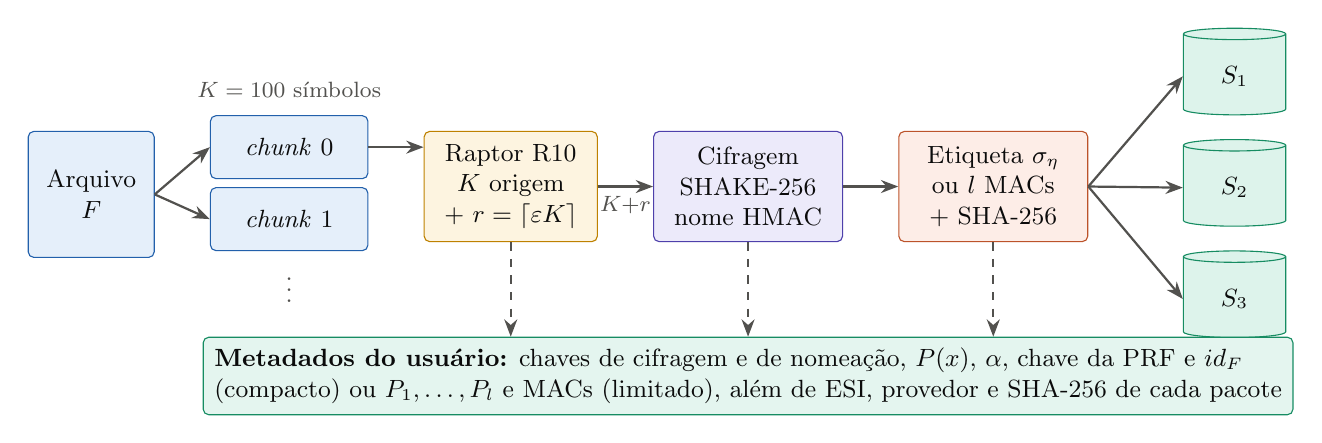
\begin{tikzpicture}[node distance=5mm and 7mm]
	\node[caixa=serieA, minimum width=16mm, minimum height=16mm] (arquivo) {Arquivo\\$F$};
	% Chunks
	\node[caixa=serieA, right=of arquivo, minimum width=20mm, yshift=6mm] (ch0) {\emph{chunk} 0};
	\node[caixa=serieA, below=1mm of ch0, minimum width=20mm] (ch1) {\emph{chunk} 1};
	\node[below=0mm of ch1, text=tintaSec] (chd) {$\vdots$};
	\draw[seta] (arquivo.east) -- (ch0.west);
	\draw[seta] (arquivo.east) -- (ch1.west);
	\node[rotulo, above=1mm of ch0] {$K = 100$ símbolos};

	% Codificação de um chunk
	\node[caixa=serieD, right=of ch0, minimum width=22mm, yshift=-5mm, minimum height=14mm] (rq) {Raptor R10\\$K$ origem\\$+\ r = \lceil \varepsilon K \rceil$};
	\draw[seta] (ch0.east) -- (rq.west |- ch0.east);
	\node[caixa=serieE, right=of rq, minimum width=24mm, minimum height=14mm] (selo) {Cifragem\\SHAKE-256\\nome HMAC};
	\node[caixa=serieB, right=of selo, minimum width=24mm, minimum height=14mm] (prova) {Etiqueta $\sigma_\eta$\\ou $l$ MACs\\+ SHA-256};
	\draw[seta] (rq) -- node[rotulo, below] {$K{+}r$} (selo);
	\draw[seta] (selo) -- (prova);

	% Provedores
	\node[servidor, right=12mm of prova, yshift=14mm] (s1) {$S_1$};
	\node[servidor, below=3mm of s1] (s2) {$S_2$};
	\node[servidor, below=3mm of s2] (s3) {$S_3$};
	\draw[seta] (prova.east) -- (s1.west);
	\draw[seta] (prova.east) -- (s2.west);
	\draw[seta] (prova.east) -- (s3.west);

	% Metadados do usuário
	\node[caixa=serieC, below=12mm of selo, minimum width=70mm, align=left] (meta) {%
		\textbf{Metadados do usuário:} chaves de cifragem e de nomeação, $P(x)$, $\alpha$, chave da PRF e $id_F$\\
		(compacto) ou $P_1, \ldots, P_l$ e MACs (limitado), além de ESI, provedor e SHA-256 de cada pacote};
	\draw[seta, dashed] (rq.south) -- (rq.south |- meta.north);
	\draw[seta, dashed] (selo.south) -- (meta.north -| selo.south);
	\draw[seta, dashed] (prova.south) -- (prova.south |- meta.north);
\end{tikzpicture}

	\end{adjustbox}
	\caption{Fluxo de Codificação e Distribuição do HyBolt: cada \emph{chunk} é codificado com o R10, cada pacote é cifrado e recebe o material de prova, e os pacotes são distribuídos entre os provedores, enquanto o usuário mantém apenas os metadados.}
	\label{fig:fluxo}
\end{figure*}

\paragraph{MAC derivado e desafios.} Pela Equação~\eqref{eq:suporte}, o MAC esperado de qualquer pacote, inclusive de símbolos de reparo gerados posteriormente, é $h_{\eta,j} = \bigoplus_{i \in X_\eta} h_{i,j}$, de modo que o usuário mantém apenas $n \cdot l$ MACs e não precisa armazenar a composição dos pacotes. Cada polinômio de desafio é obtido por amostragem com rejeição e validado pelo teste de irredutibilidade de Rabin \cite{rabin1980probabilistic}; como $2^{127} - 1$ é primo, todo polinômio irredutível de grau $\lambda = 127$ é primitivo.

\paragraph{Auditoria ponderada.} A resposta original, o XOR dos pacotes desafiados, permite que dois pacotes alterados pelo mesmo erro $e(x)$ se anulem. O HyBolt pondera cada pacote por uma potência secreta de $x$, com expoentes distintos $k_\eta < 2^{32}$:
\begin{equation}
A(x) = \textstyle\left(\sum_{\eta} x^{k_\eta} c_\eta(x)\right) \bmod P_j(x).
\end{equation}
Como $x$ tem ordem $2^\lambda - 1$ módulo um polinômio primitivo, o cancelamento exigiria $k_a \equiv k_b \pmod{2^\lambda - 1}$, o que é impossível.

\paragraph{Redistribuição.} Um pacote corrompido é substituído por um símbolo de reparo de ESI inédito $t$, cujo suporte o usuário expressa, por eliminação gaussiana em $GF(2)$, como a diferença simétrica dos suportes de um subconjunto $Q$ de pacotes íntegros; o novo pacote é $c_t = \bigoplus_{q \in Q} c_q$. O \emph{chunk} nunca é decodificado, e cada reparo transfere, em média, 49 pacotes, cerca de 320~KB.

\paragraph{Esquema compacto.} O modelo limitado revela cada $P_j$ ao provedor e, portanto, admite apenas $l$ auditorias e exige do usuário memória proporcional ao arquivo. Inspirado em Shacham e Waters \cite{shacham2008compact}, o HyBolt associa a cada pacote a etiqueta $\sigma_\eta = (c_\eta \bmod P) + f_K(id_F, i, \eta)$, em que $P$ é um polinômio primitivo secreto e $f_K$ uma função pseudoaleatória (HMAC-SHA-256). O provedor responde com combinações lineares $\mu = \sum \nu_\eta c_\eta$ e $\tau = \sum \nu_\eta \sigma_\eta$, que o usuário verifica sem revelar $P$. As auditorias tornam-se ilimitadas, e as chaves ocupam 64 bytes.

\paragraph{Ocultação da estrutura.} Como o R10 não é MDS e sua estrutura é pública, um adversário pode corromper os sete pacotes que contêm um mesmo símbolo de origem e tornar o \emph{chunk} irrecuperável, contra os $r + 1 = 26$ que um código MDS exigiria. Para impedir esse ataque, cada pacote é cifrado com um fluxo SHAKE-256 e armazenado sob um nome pseudoaleatório, seguindo \cite{juels2007pors,bowers2009proofs}; a cifragem é linear em $GF(2)$ e preserva o MAC derivado.

\section{Metodologia e Ambiente Experimental}
\label{sec:metodologia}

Para que a comparação não dependa de medidas publicadas em outro equipamento, os Online Codes foram implementados no próprio HyBolt e executados no mesmo fluxo que o R10, variando apenas o código \emph{fountain}. O R10 foi implementado a partir da norma e validado byte a byte contra a biblioteca independente \texttt{gofountain}, e a aritmética em $GF(2)[x]$ foi implementada como extensão em C. Os experimentos foram executados em um Intel Core i7-11390H com 8~GB de memória, sob WSL2 e Python~3.13, com três provedores simulados por diretórios locais, o que exclui a latência de rede. Utilizaram-se os parâmetros padrão ($\lambda = 127$, $K = 100$, $\varepsilon = 0{,}25$, $l = 40$) e dados pseudoaleatórios, e cada arquivo decodificado foi comparado byte a byte com o original. As simulações de recuperação utilizaram 2.000, 1.000 e 200 repetições para $K = 10$, 100 e 1.000, e todos os resultados são reproduzidos pelo script \texttt{scripts/thesis\_benchmarks.py}.

\section{Resultados}
\label{sec:resultados}

\paragraph{\emph{Overhead} de recepção.} A Figura~\ref{fig:overhead} e a Tabela~\ref{tab:overhead} comparam o número de símbolos necessário à recuperação. O R10 exigiu um número aproximadamente constante de símbolos excedentes, de 1,4 a 2,7, que corresponde a 1,8\% de $K$ no \emph{chunk} padrão, contra 34\% dos Online Codes. O RaptorQ recuperou com exatamente $K$ símbolos em mais de 99\% dos casos, mas, como discutido, é incompatível com o MAC homomórfico.

\begin{figure}[t]
	\centering
	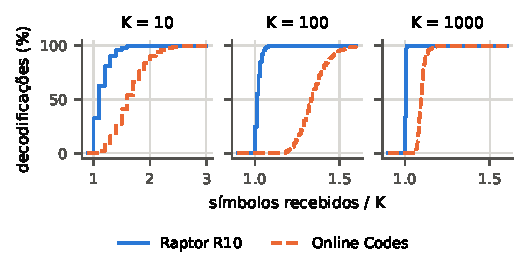
\includegraphics[width=\columnwidth]{figures/reception_overhead.pdf}
	\caption{Fração das decodificações concluídas em função do número de símbolos recebidos, normalizado por $K$.}
	\label{fig:overhead}
\end{figure}

\begin{table}[t]
	\centering
	\caption{Símbolos adicionais médios necessários à recuperação, em porcentagem de $K$.}
	\label{tab:overhead}
	\small
	\begin{tabular}{@{}lrrr@{}}
		\toprule
		\textbf{Código} & $K = 10$ & $K = 100$ & $K = 1.000$ \\
		\midrule
		Raptor R10   & 14,1\% & 1,8\%   & 0,27\%   \\
		RaptorQ      & 0,05\% & 0,005\% & 0,0005\% \\
		Online Codes & 64,9\% & 34,3\%  & 9,7\%    \\
		LT Codes     & 56,4\% & 32,5\%  & 17,3\%   \\
		\bottomrule
	\end{tabular}
\end{table}

\paragraph{Tolerância a perdas.} A Figura~\ref{fig:perdas} apresenta a recuperação de um \emph{chunk} em função da fração de pacotes perdidos. Com $\varepsilon = 0{,}25$, o R10 tolerou a perda de 18 dos 125 pacotes (14,4\%) em pelo menos 99\% dos casos, próximo do limite MDS de 20\%. Os Online Codes, embora armazenem 143 pacotes por \emph{chunk}, tornaram-se irrecuperáveis em 7,4\% dos casos com a perda de um único pacote e em 42\% com a perda de cinco. Com $\varepsilon = 0{,}5$, as perdas toleradas foram de 43 pacotes com o R10 e de apenas dois com os Online Codes.

\begin{figure}[t]
	\centering
	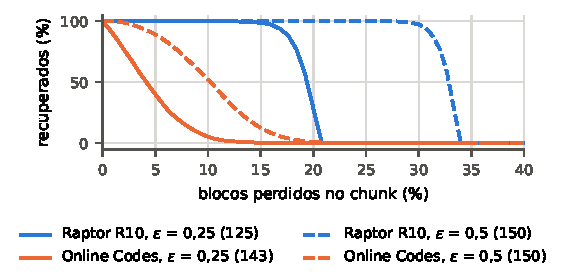
\includegraphics[width=\columnwidth]{figures/codec_loss.pdf}
	\caption{\emph{Chunks} de $K = 100$ símbolos recuperados em função da fração de pacotes perdidos, com R10 e Online Codes, estimados por 4.000 ordens aleatórias.}
	\label{fig:perdas}
\end{figure}

\paragraph{Desempenho.} O custo dos dois códigos mostrou-se equivalente: a mediana foi de 2,8~ms para codificar e 3,5~ms para decodificar um \emph{chunk} com o R10, contra 2,6 e 3,2~ms com os Online Codes. A diferença está no volume de dados: os Online Codes armazenam 1,45 vez o arquivo, contra 1,27, e a decodificação recebeu em média 136,3 pacotes por \emph{chunk}, contra 101,5, o que tornou a decodificação sem prova de 23\% a 75\% mais lenta. No esquema compacto, um arquivo de 64~MiB foi codificado em 2,2~s (29~MiB/s), e os metadados do usuário convergiram para 2,7\% do arquivo, contra 154\% do esquema limitado para 1~MiB. A redução polinomial em C calculou o MAC de um bloco de 40~KiB em 0,11~ms, ao passo que a implementação original do HySAIL reportava 62~s \cite{amaral2013hysail}, em outro equipamento.

\paragraph{Auditoria e ocultação.} Com 5,1\% dos pacotes de um provedor corrompidos, uma amostra de 50 pacotes detectou a corrupção em 96\% das rodadas, em concordância com a probabilidade teórica $1 - (1 - \beta)^s$. A Figura~\ref{fig:ataque} mostra o efeito da ocultação: para um arquivo de 1~GiB, a fração de pacotes que o adversário precisa corromper para que a perda do arquivo se torne possível passa de 0,0034\% para cerca de 4\%, e para que se torne mais provável que a recuperação, para 8,5\%. Com 4\% de corrupção, uma auditoria de 50 pacotes por provedor a detecta em ao menos um dos três provedores com probabilidade superior a 99,8\%, o que permite iniciar a Redistribuição antes da perda de dados.

\begin{figure}[t]
	\centering
	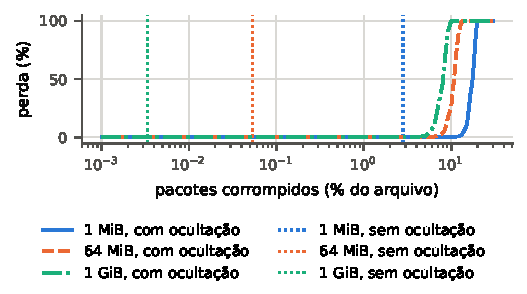
\includegraphics[width=\columnwidth]{figures/targeted_attack.pdf}
	\caption{Probabilidade de perda do arquivo em função da fração de pacotes corrompidos, com ocultação (corrupção uniforme) e sem ocultação (linhas pontilhadas: ataque dirigido a um \emph{chunk}).}
	\label{fig:ataque}
\end{figure}

\section{Aspectos Éticos}
\label{sec:ethics}

A pesquisa não envolveu seres humanos nem dados pessoais: todos os experimentos utilizaram arquivos de bytes pseudoaleatórios e provedores simulados localmente, razão pela qual não foi necessária a apreciação por comitê de ética. Os ataques avaliados foram executados apenas sobre dados sintéticos, com o propósito de dimensionar as defesas propostas.

\section{Conclusão}
\label{sec:conclusao}

Este trabalho mostrou que a substituição dos Online Codes pelo Raptor R10 preserva as propriedades estruturais do HySAIL, o MAC homomórfico e a Redistribuição local, que o RaptorQ não preservaria, e que, com o mesmo custo computacional, o R10 reduz o \emph{overhead} de recepção de 5 a 36 vezes e eleva a tolerância a perdas de um \emph{chunk} de nenhum para 14\% dos pacotes. O esquema compacto elimina as limitações do modelo limitado, e a ocultação da estrutura eleva em mais de três ordens de grandeza a corrupção necessária para destruir um arquivo grande.

Como limitações, o R10 não é MDS, o que torna inadequados \emph{chunks} pequenos; com três provedores, tolerar a saída de um deles exige $\varepsilon \ge 0{,}6$; e a garantia de extração do esquema compacto ainda deve ser formalizada. Trabalhos futuros incluem essa formalização, a verificação pública por auditores delegados \cite{armknecht2021outsourcing}, a otimização da gravação e da cifragem dos pacotes, que dominam o tempo de codificação, e a avaliação em provedores de nuvem reais.

\begin{declarations}

\begin{contributions}
O primeiro autor concebeu a proposta, implementou o HyBolt, conduziu os experimentos e redigiu o manuscrito. O segundo autor supervisionou a pesquisa e revisou o manuscrito. Todos os autores leram e aprovaram a versão final.
\end{contributions}

\begin{interests}
Os autores declaram que não têm nenhum conflito de interesses.
\end{interests}

\begin{materials}
O código-fonte do HyBolt, os scripts de experimentos e os dados brutos que reproduzem as figuras deste artigo estão disponíveis no repositório do projeto.
\end{materials}

\begin{furtherinformation}
Este artigo resume a dissertação de mestrado que propôs o HyBolt. Ferramentas de IA generativa foram utilizadas como apoio à redação, e todo o conteúdo foi revisado pelos autores.
\end{furtherinformation}
\end{declarations}

\bibliographystyle{apalike-sol}
\bibliography{refs}

\end{document}
